% options:
% thesis=B bachelor's thesis
% thesis=M master's thesis
% czech thesis in Czech language
% slovak thesis in Slovak language
% english thesis in English language
% hidelinks remove colour boxes around hyperlinks

\documentclass[thesis=B,czech]{FITthesis}[2013/05/06]

\usepackage[utf8]{inputenc} % LaTeX source encoded as UTF-8

\usepackage{placeins}
\usepackage{graphicx} %graphics files inclusion
% \usepackage{amsmath} %advanced maths
% \usepackage{amssymb} %additional math symbols

\usepackage{dirtree} %directory tree visualisation

\usepackage{minted}
\renewcommand\listingscaption{Ukázka kódu}
\renewcommand\listoflistingscaption{Seznam ukázek kódu}

% % list of acronyms
% \usepackage[acronym,nonumberlist,toc,numberedsection=autolabel]{glossaries}
% \iflanguage{czech}{\renewcommand*{\acronymname}{Seznam pou{\v z}it{\' y}ch zkratek}}{}
% \makeglossaries

\newcommand{\tg}{\mathop{\mathrm{tg}}} %cesky tangens
\newcommand{\cotg}{\mathop{\mathrm{cotg}}} %cesky cotangens

% % % % % % % % % % % % % % % % % % % % % % % % % % % % % %
% ODTUD DAL VSE ZMENTE
% % % % % % % % % % % % % % % % % % % % % % % % % % % % % %

\department{Katedra softwarového inženýrství}
\title{Kolaborativní tvorba LaTeX dokumentů s podporou Gitu}
\authorGN{Filip} %(křestní) jméno (jména) autora
\authorFN{Chalupa} %příjmení autora
\authorWithDegrees{Filip Chalupa} %jméno autora včetně současných akademických titulů
\supervisor{Ing. Tomáš Kalvoda, Ph.D.}
\acknowledgements{Doplňte, máte-li komu a za co děkovat. V~opačném případě úplně odstraňte tento příkaz.}
\abstractCS{V~několika větách shrňte obsah a přínos této práce v~češtině. Po přečtení abstraktu by se čtenář měl mít čtenář dost informací pro rozhodnutí, zda chce Vaši práci číst.}
\abstractEN{Sem doplňte ekvivalent abstraktu Vaší práce v~angličtině.}
\placeForDeclarationOfAuthenticity{V~Praze}
\declarationOfAuthenticityOption{4} %volba Prohlášení (číslo 1-6)
\keywordsCS{LaTeX, Git, verzování, kolaborace, přístupnost}
\keywordsEN{LaTeX, Git, versioning, collaboration, accessibility}

\begin{document}

% \newacronym{CVUT}{{\v C}VUT}{{\v C}esk{\' e} vysok{\' e} u{\v c}en{\' i} technick{\' e} v Praze}
% \newacronym{FIT}{FIT}{Fakulta informa{\v c}n{\' i}ch technologi{\' i}}

%\chapter{Úvod}
Častým scénářem při tvorbě různých skript, vědeckých článků, informačních podkladů, prezentací je spolupráce několika osob. V takových týmech je důležitá komunikace mezi jednotlivými členy a sdílení aktuálního rozpracovaného díla.

\section{Hypotéza}

K dispozici je spousta nástrojů, jejichž smyslem je tvorbu ve skupině usnadnit; velké množství, různorodost, a v některých případech větší komplexita však značně komplikuje jejich nasazení. Důsledkem je uchýlení se k více známým a z podstaty primitivnějším řešením, například přeposílání rozdělané práce přes e-mail nebo předávání podkladů přes externí uložiště a nedělání záloh předešlých verzí. Tým tím ztrácí na efektivitě, což se může podepsat na kvalitě díla a zbytečném protahování tvorby.

\section{Terminologie}

\subsection{\LaTeX}

\uv{LaTeX je komplexní systém pro sazbu dokumentů. Stará se tedy o zalamování textu do odstavců, vkládání obrázků, seznamů, nadpisů, matematických výrazů, rozdělování dokumentu na jednotlivé stránky, ligatury, "vdovy" a "sirotky", odsazení\ldots} \cite{latex-def}

\subsection{Git}

Verzovací systém s podporou více uživatelů a ukládáním projektu na vzdálený server například v internetu.

\subsection{Verzování}

Sledování projektu s průběžným ukládání změn pro zpětné dohledání přidaných či odebraných řádků v textovém souboru, případně přidání či odebrání binárního souboru.

\subsection{Kolaborace}

Spolupráce více osob na jednom projektu.

\subsection{Přístupnost}

Umožnění práce se složitějšími nástroji pro osoby s nedostatečnou znalostí ovládání.

\section{Struktura práce}

Následující kapitoly se budou zabývat ověřením hypotézy pomocí uživatelského průzkumu a analýzou existujících řešení, návrhem vlastního řešení s požadavky a volbou prostředků pro jeho implementaci, podrobnějším rozborem tvorby uživatelského rozhraní, distribucí aplikace, testováním, poznatky ohledně knihovny NodeGit, návrhy na další vývoj a závěrečným shrnutím.


%\chapter{Cíl práce}
Tristní situaci přednesenou v úvodu je tedy žádoucí vyřešit buď vyškolením účastníků týmu, nebo představením nového nástroje, který disponuje funkcemi komplexních nástrojů, ale zároveň je jednoduchý na použití i pro začátečníka, což je i cílem této práce, zhotovení nové aplikace určené pro operační systémy primárně Windows a Linux. K jeho dosažení je potřeba provést podrobnější analýzu současného stavu. Je tedy nutné proniknout do pracovních postupů autorů, jimž práce v týmu psaním v LaTeXu způsobuje potíže. Na základě například dotazníků či rozhovorů. Tímto se dostaneme do druhé fáze, kdy bude potřeba navrhnout principy aplikace, její nároky na uživatelské rozhraní a podporované funkce. Dále dojde k implementaci vybraného návrhu a na závěr k otestovaní dotazovanými z analytické části.


%\chapter{Cílová skupina uživatelů}

Záměrem vzniklé aplikace je vytvoření prostředí pro snadnou správu, tj. sdílení a verzování, textových dokumentů.
% TODO: co je to textový dokument
Důraz je kladen na formát LaTeXu, avšak nejedná se o omezení. Aplikace funguje jako nadstavba nad systémem Git, takže umožňuje spolupráci více autorů, kde každý nemusí aplikaci používat. Vzhledem k tomu, že Git je velmi populární nástroj,
% @TODO: doplnit nějakou statistiku
někteří autoři dokumentů ho na sdílení a verzování použíbají již teď. Pro snadnou práci v libovolném týmu, kde se mohou nacházet uživatelé s i bez aplikace, je tento scénář podporován. Není vytvořeno ani žádné omezení na službu, která sprostředkovává funkci vzdáleného serveru.
% @TODO: doplnit referenci, co je vzdálený server
Je tedy možné využít například veřejný Github, Bitbucket či třeba provozovat GitLab na vlastním serveru. Vzdálený server slouží jako prostředník mezi autory, kdy na něj jsou ukládány průběžně verze všech autorů. Libovolný autor tak může přejímat aktuální sdílenou verzi a dále ji rozšiřovat. Není však po úplně celou dobu závislý na připojení k internetu, tj. na připojení ke vzdálenému serveru. Připojení je pouze vyžadováno v okamžiku, kdy autor chce nahrát své změny, poskytnout ostatním autorům a zároveň zazálohovat, nebo stáhnout nové úpravy ostatních.
% TODO: vysvětlit, co jsou to změny
Každopádně i bez připojení má autor lokálně uloženou poslední známou historii změn, na které může pracovat. S další synchronizací se pak rozhodne, jestli své změny poskytne i ostatním. Může se totiž stát, že v době bez spojení například někdo rozvinul dokument jiným směrem a místní změny tak nemusí být dále užitečné nebo nemusí být kompatibilní s aktualizovaným stavem dokumentu. V takové situaci aplikace vyzve autora k vyřešení takzvaných merge confliktů, kdy je potřeba některé změny doupravit.


%\chapter{Současný stav}
Jako ověření, že vytváření nové aplikace má význam, byly prozkoumány současné možnosti, které si kladou za cíl řešení stejného problému. K dispozici jsou například online nástroje ShareLaTeX a Overleaf. První zmíněný, „Online LaTeX editor snadný k použití s možností spolupráce více autorů“ {cit2}, se sice hned na úvodní stránce chlubí překladem do češtiny, který je ale nekompletní a práce s ním je tak často matoucí, z textů není jasné, co se zrovna děje, co se od uživatele očekává a jakým způsobem má pracovat. K tomu vyžaduje vysoký měsíční poplatek {cit3} za zpřístupnění většiny funkcí. Druhá služba, Overleaf, překlad do češtiny nenabízí vůbec, což není nutné považovat za nedostatek, protože požadavkem není řešení konkrétně pro české prostředí. Chybí však funkce pro procházení změn v historii projektu.

Obě služby trpí omezením, že se nelze dostat k úpravám projektu mimo ně. Uživatel nemůže tvořit ve svém oblíbeném editoru, musí si vystačit s online editorem, který navíc nenabízí žádnou offline variantu.

Alternativním přístupem je třeba verzovací systém Git, jež je zejména pro začátečníky s tímto systémem příliš komplikovaný.

těm psům


hypotéza?

\chapter{Průzkum}

Po vymezení základní hypotézy byly provedy dva průzkumy. První se zaměřením na vzorek možných uživatelů. Jeho cílem bylo ověřit, jestli problém skutečně existuje a jaké jsou potenciální nároky na jeho řešení. Druhý prozkoumával již existující nástroje pro práci v týmu s \LaTeX{em} a jejich nedostatky.

\section{Uživatelé}

Formou osobních rozhovorů proběhly diskuze s pěti učiteli z ČVUT zaměřujících se převážně na tvorbu materiálů s tématikou matematiky. Každá diskuze byla zahájena stručným představením a dále otázkami, jaké materiály učitel tvoří a za pomoci jakých nástrojů. Zbytek se odvíjel podle odpovědí na tyto první dva dotazy. Volba respondentů vycházela z doporučení vedoucího této bakalářské práce a z rohodnutí autora nevyhledávala další, protože všechny ověpovědi hypotézu problému podporovaly a zároveň byly dostatečně různorodé. Následuje výčet poznatků od všech pěti respondentů z prosince roku 2015.

\subsection{Respondent A}

\begin{itemize}
	\item Ing. Daniel Dombek, Ph.D.
	\item Odborný asistent na katedře aplikované matematiky \cite{kam},
	\item píše zejména handouty pro předmět BI-ZDM\footnote{\url{https://edux.fit.cvut.cz/courses/BI-ZDM/start}},
	\item práci se spoluautory sdílí přes fakultní GitLab\footnote{\url{https://gitlab.fit.cvut.cz/}},
	\item poznámky a další komunikaci posílá přes e-mail,
	\item běžně pracuje sám či až se čtyřmi lidmi,
	\item zálohuje, verzuje i práci, na které dělá jediný,
	\item se spolupracujími je domluvený, že nemění v jednu chvíli stejné soubory kvůli vyvarování se možných kolizí,
	\item píše v TeXstudio\footnote{\url{http://www.texstudio.org/}},
	\item sdílí pomocí nástroje TortoiseGit\footnote{\url{https://tortoisegit.org/}} a pluginu pro Git do Total Commanderu\footnote{\url{https://github.com/Darthholi/WDX\_GitCommander}},
	\item setkává se s problémem hromadění tabů, znaků pro odsazení, který je pravděpodobně způsoben různou konfigurací editorů ostatních autorů, kdy možná některý převádí mezery na začátku řádků pro přehledné odsazení zdrojového textu na neúměrný počet tabů,
	\item nevyhovují mu přebytečné neviditelné znaky na koncích řádků,
	\item v Gitu vytváří jeden commit za svou celodenní práci,
	\item má zájem sledovat historii o jeden commit zpět.
\end{itemize}


\subsection{Respondent B}

\begin{itemize}
	\item Ing. Štěpán Starosta, Ph.D.
	\item Odborný asistent na katedře aplikované matematiky \cite{kam},
	\item sdílí kancelář s prvním respondentem, takže je přítomný u předchozího rozhovoru a ve většině se na odpovědích shodne
	\item zmiňuje konkurenci Overleaf\footnote{\url{https://www.overleaf.com/}}, ale není jejím aktivním uživatelem,
	\item občas řeší konflikty, když méně zkušený spoluautor v Gitu zapomene před zahájením své práce stáhnout aktuální úpravy ostatních,
	\item také mimo Git komunikuje přes e-maily,
	\item píše v Sublime Text s pluginem GitGutter\footnote{\url{https://github.com/jisaacks/GitGutter}},
	\item má spoustu pomocného kódu, který sdílí napříč různými projekty, ale neví, jak ho efektivně vždy přenášet,
	\item rád používá pro zvýraznění změn Latexdiff\footnote{\url{https://www.ctan.org/pkg/latexdiff}}
	\item chtěl by nějak do \LaTeX{u} dostat poznámky z Gitu například o aktuální revizi, aby získal lepší přehled o již vytištěných verzích a mohl je snadno zpětně spárovat s historií commitů.
\end{itemize}


\subsection{Respondent C}

\begin{itemize}
	\item Mgr. Michal Kupsa, Ph.D.
	\item Odborný asistent na katedře aplikované matematiky \cite{kam},
	\item píše články o deseti až dvaceti stranách,
	\item zkušenosti má s verzovacím nástrojem Git a SVN,
	\item pracuje v Emacs\footnote{\url{https://www.gnu.org/software/emacs/}},
	\item s týmem také komunikuje přes e-mail,
	\item ve správci úkolů (issue tracker) na GitLabu mu chybí zobrazování vzorců, protože GitLab je neumí příliš dobře,
	\item možnost přehledu historie vnímá jako pozitivum.
\end{itemize}


\subsection{Respondent D}

\begin{itemize}
	\item Ing. Daniel Vašata, Ph.D.
	\item Odborný asistent na katedře aplikované matematiky \cite{kam},
	\item píše v Sublime Text s pluginem LaTeXTools\footnote{\url{https://github.com/SublimeText/LaTeXTools}},
	\item má zkušenost s Gitem a SVN,
	\item pro pohodlnější práci s Gitem používá SmartGit\footnote{\url{http://www.syntevo.com/smartgit/}},
	\item commity vytváří na konci dne, což mu vychází na větší logickou část,
	\item zajímá ho historie na úrovni jednotlivých souborů,
	\item je zaujatý nástrojem Latexdiff.
\end{itemize}


\subsection{Respondent E}

\begin{itemize}
	\item RNDr. Ondřej Suchý, Ph.D.
	\item Odborný asistent na katedře teoretické informatiky \cite{kti},
	\item tvoří prezentace, píše články, úlohy pro středoškoláky,
	\item účastní se v týmech do sedmi lidí,
	\item výjimkou je tým na tvorbu úloh pro středoškoláky, jenž se skládá z dvanácti lidí,
	\item práci sdílí výhradně přes SVN,
	\item s \uv{významnějšími} autory přes Dropbox\footnote{\url{https://www.dropbox.com}}, avšak zde mu nevyhovuje správa verzí,
	\item nasazení Gitu vidí jako zbytečnou komplikaci pro již zaběhnuté prostředí,
	\item navíc každý úkon je pro něj v Gitu dvakrát složitější než v SVN i kvůli náročnějšímu řešení merge,
	\item komunikuje přes IRC či e-mail, který občas obohatí o diff export z SVN,
	\item v rozdílech mezi jednotlivými commity vyžaduje zvýraznění na úrovni změněných slov, standardní rozlišování pouze řádků je nedostatečné,
	\item píše v Kile\footnote{\url{http://kile.sourceforge.net/}}, na kterém si chválí automatické doplňování a náhledy.
\end{itemize}

Kromě respondentů byl zdrojem podnětů i samotný vedoucí práce, Ing.~Tomáš Kalvoda,~Ph.D. Odborný asistent na katedře aplikované matematiky, který průběžně usměrňoval vývoj řešení. Přišel s původní hypotézou.

\section{Existující řešení}

\section{Shrnutí}

\subsection{Rozhovory}

Dotazování mají většinout nějakou zkušenost s prací s Gitem, ale kvůli složitému ovládání ho často nepoužívájí spávně nebo netěží ze všech jeho výhod. Například je nevhodné dělat commit pouze na konci dne, pokud by měl obsahovat více změn netvořících jeden malý logický celek. Dobrý commit pomáhá všem účastníkům se v projektu lépe orientovat a změny dále upravovat a rozvíjet. V týmech se objevují různě zkušení uživatelé. Někteří zanechávají nevhodné neviditelné znaky na koncích řádků nebo převádí taby na mezery a obráceně, nerespektují domluvený styl zdrojového textu. Každý dotazovaný používá editor vlastní volby z různých důvodů. S výběrem jsou spokojení; panuje pochopitelná neochota učit se s novým editorem z časových důvodů a kvůli chybějícím funkcím. Je zájem o verzování a usnadnění sdílení napříč týmem.

\subsection{Existující řešení}

Dostupné nástroje značně omezují týmy tím, že vyžadují neustálé připojení k internetu a užívání jediného editoru. Chybí dobrá podpora češtiny. Historie změn nejsou přehledné.


\chapter{Řešení}
Řešením je nová aplikace, která je schopná běžet na různých cílových zařízení, se systémem Windows nebo Linux, tak, aby vystihla různorodost zařízení členů týmu (systém, editor LaTeXu), ale zároveň nenutila všechny členy k jejímu aktivnímu využívání. Čtyřčlenný tým může vypadat třeba tak, že jeden autor pracuje na svém počítači se systémem Windows s pomocí nové aplikace, podobně další dva členové se systémem Linux a čtvrtý člen s pokročilou znalostí verzovacího systému Git nemusí novou aplikaci používat vůbec a stejně může bez omezení spolupracovat se zbytkem týmu. Aplikace tedy musí být schopná komunikovat se systémem Git, který splňuje požadavek na zálohování a verzování.


\chapter{Grafické rozhraní}

Grafické rozhraní je tvořené trojicí HTML, CSS a JavaScript, což jsou pilíře současných webových stránek. Velká část Aplikace by tedy mohla běžet v~moderním webovém prohlížeči jako je například Google Chrome, jehož jádro pro zobrazování stránek je totožné jako jádro Electronu, který se stará o~vykreslování obsahu okna Aplikace. Funkcionalita, kterou Electron nabízí navíc, je například přístup k~souborovému systému uživatele, systémovým voláním či spouštění vlastních kompilovaných programů například z~jazyka C. Tato kapitola se dále bude zabívat pouze částí Aplikace, která je pro uživatele viditelná v~hlavním okně či v~prostoru pro upozornění.

Ve fázi prototypování byl zvolen framework Boostrap\footnote{\url{https://getbootstrap.com/}} třetí verze, jenž nabízel velmi známe rozhraní jak pro uživatele, tak pro kodéra. Díky němu bylo možné velmi rychle nastínit strukturu Aplikace a přidat tlačítka a textová pole pro uživatelský vstup, která spouštěla kritické útržky kódu, pro testování hlavního konceptu či funkcionality podpůrné knihovny pro práci s~Gitem v~JavaScriptu. V~prototypovací fázi se ukázalo, že Bootstrap nebude příliš vhodný framework pro další vývoj. Při tvorbě složitějších komponent začal rychle prezentovat své nedostatky. Jedním příkladem budiž skladba i jednoduchých prvků, která vyžaduje přemíru obsahu, jenž není pro běžného uživatele vidět, ale je kritický pro dostupnost webu například při indexaci vyhledávači, což pro Aplikaci je naprosto zbytečná vlastnost. Zároveň nevznikl projekt, který by kvalitně tyto složité struktury abstrahoval do jednodušších, snáze použitelných. Nechť jako ukázka slouží React-Bootstrap\footnote{\url{https://react-bootstrap.github.io/}}, který se může pyšnit slušnými deseti tisíci hvězdiček na GitHubu a aktivním vývojem. Byť práci s~Bootrapem velmi zjednodušuje, zatím neobsahuje dostatečné množství připravených komponent. Druhým a zásadnějším nedostatkem je chybějící podpora pro udržování stavu, protože Bootstrap je spíše orientovaný na klasické weby, které se generují na serveru a uživateli se tak často při změně projevují probliknutím při změně, které je způsobené prodlevou při komunikaci se serverem a přerenderování celé stránky, což by opět vyřešilo dotažení React-Boostrapu, kdy by obsahoval všechny původní komponenty z~Bootrapu.

Na místě bylo tedy najít jiné řešení, které by usnadnilo tvorbu rozhraní s~požadavky na snadné uživání, dostatečnou databázi předpřipravených komponent a jednoduché zakomponování nějakého systému pro uchovávání stavu. Dalším kandidátem se stal React Desktop\footnote{\url{http://reactdesktop.js.org/}}, který splňoval základní požadavky a jako bonus nabízel vzhled, který byl šitý na míru různým systémům. Měl vlastní vzhled pro macOS a Windows 10, což se nakonec ukázalo jako nevýhoda, protože, i přes to, že na zmíněných systémech by poskytoval výborný uživatelský zážitek daný známostí prostředí, oba vzhledy byly tak specifické, že by nefungovaly v~kontextu ostatních linuxových systémů.

% @TODO: rozepsat více
Vítězem při volbě se nakonec stal Materia-UI\footnote{\url{http://www.material-ui.com/}}, který řeší nedostatky dříve zkoumaných možností. Více o~něm v~následující sekci.

\section{Material-UI}

Tento framework je implementací Material Designu od společnosti Google \cite{material-from-google}. Material-UI obsahuje spoustu připravených komponent, které jsou na míru šité pro tvorbu aplikací díky rozsáhle studii Googlu, která je pomocí zásad a instrukcí popsaná na vlastním webu\footnote{\url{https://material.io/guidelines/}}. Grafické rozhraní Aplikace je složeno z těchto komponent. Jedná se zejména o Appbar, Avatar, různé varianty pro Button, Card, Dialog, Drawer, Progress, formulářové prvky, Snackbar, Tabs a ikony\footnote{\url{https://material.io/icons/}}. Následují obrázkové ukázky:

\FloatBarrier

\begin{figure}[ht]
	\centering
	
\includegraphics[scale=0.5]{sections/ui/images/Appbar.png}
	\caption{Appbar}
	\label{fig:appbar}
\end{figure}

\begin{figure}[ht]
	\centering
	
\includegraphics[scale=0.5]{sections/ui/images/Avatar.png}
	\caption{Avatar}
	\label{fig:avatar}
\end{figure}

\begin{figure}[ht]
	\mbox{
\includegraphics[scale=0.5]{sections/ui/images/Button-Flat.png}}   
	\hspace{12px}
	\mbox{
\includegraphics[scale=0.5]{sections/ui/images/Button-Raised.png}}
	\hspace{12px}
	\mbox{
\includegraphics[scale=0.5]{sections/ui/images/Button-Floating.png}}
	\hspace{12px}
	\mbox{
\includegraphics[scale=0.5]{sections/ui/images/Button-Icon.png}}
	\caption[Button]{Flat, Raised, Floating Action a Icon Button}
	\label{fig:buttons}
\end{figure}

\begin{figure}[ht]
\centering

\includegraphics[scale=0.5]{sections/ui/images/Tabs.png}
\caption[Tabs]{Tabs pro skrytí osahu při přidávání projektu}
\label{fig:tabs}
\end{figure}

\begin{figure}[ht]
\centering

\includegraphics[scale=0.5]{sections/ui/images/Snackbar.png}
\caption[Snackbar]{Snackbar, informační lišta ve spodní části okna o právě proběhlé akci}
\label{fig:snackbar}
\end{figure}

\begin{figure}[ht]
	\centering
	
\includegraphics[scale=0.5]{sections/ui/images/Card.png}
	\caption[Card]{Card, rámeček sloužící k seskupení souvisejícího obsahu}
	\label{fig:card}
\end{figure}

\begin{figure}[ht]
	\centering
	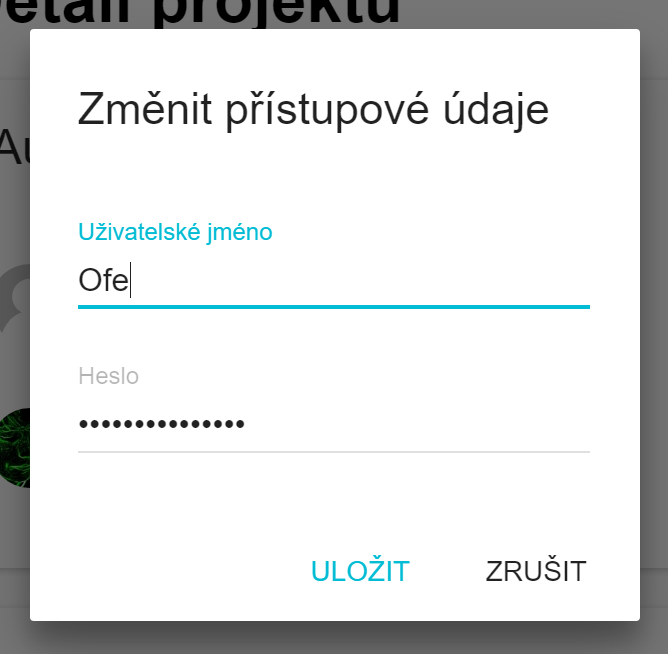
\includegraphics[scale=0.5]{sections/ui/images/Dialog.png}
	\caption[Dialog]{Dialog zobrazuje modální okna uvnitř aplikace}
	\label{fig:dialog}
\end{figure}

\begin{figure}[ht]
	\centering
	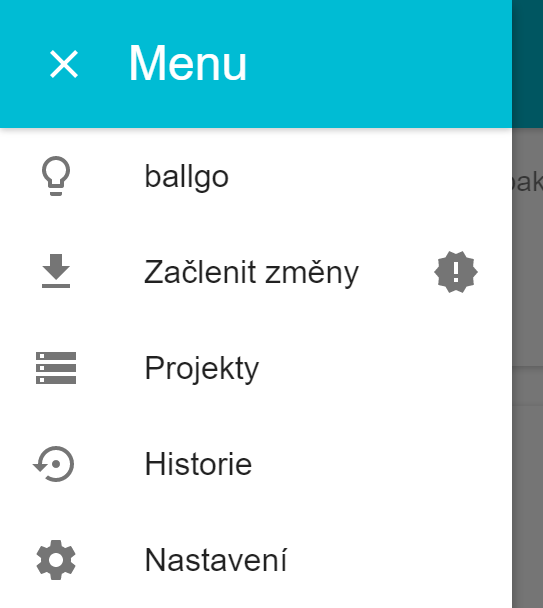
\includegraphics[scale=0.5]{sections/ui/images/Drawer.png}
	\caption[Drawer]{Drawer, boční vysouvací nabídka}
	\label{fig:drawer}
\end{figure}

\begin{figure}[ht]
	\centering
	
\includegraphics[scale=0.5]{sections/ui/images/Progress.png}
	\caption[Progress]{Animované znázornění právě probíhající akce}
	\label{fig:progress}
\end{figure}

\begin{figure}[ht]
	\mbox{
\includegraphics[scale=0.5]{sections/ui/images/TextField.png}}   
	\hspace{12px}
	\mbox{
\includegraphics[scale=0.5]{sections/ui/images/Checkbox.png}}
	\caption[TextField a Checkbox]{TextField pro uživatelův textový vstup a Checkbox pro označování souborů}
	\label{fig:form}
\end{figure}

\FloatBarrier


\section{Struktura Aplikace}

Aplikace je tvořena jediným oknem a systémovými upozorněními. Pokud uživatel chce pracovat na více projektech zároveň, může si Aplikaci na jednom počítačí otevřít několikrát naráz.


\begin{figure}[ht]
	\centering
	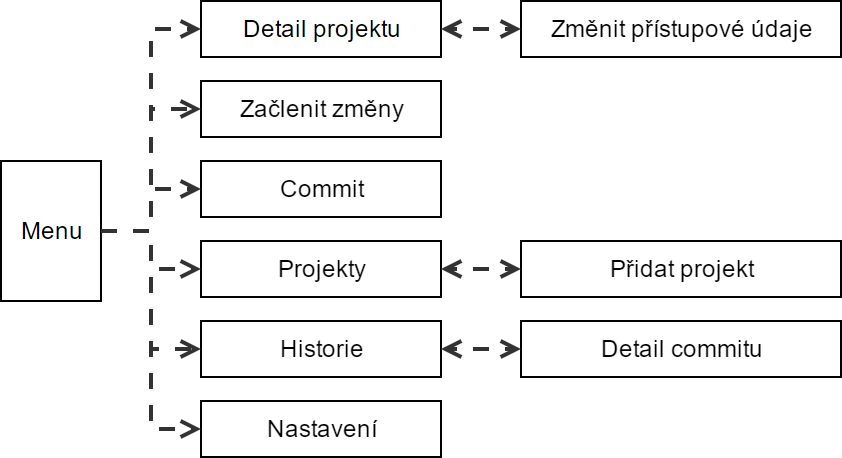
\includegraphics[width=\textwidth]{sections/ui/images/flow.png}
	\caption{Diagram struktury uživatelského rozhraní}
\end{figure}

Po levé straně se nabízí rozbalovací menu, jež může obsahovat položky detail projektu, „Commit“, „Projekty“, „Historie“ a „Nastavení“. První zmíněná položka je nahrazena názvem projektu. Vstupní obrazovkou je stránka s projekty, která se také zobrazuje vždy po spuštení aplikace. Obsahuje seznam projektů, které si uživatel do Aplikace přidal pomocí tlačítka plus (Floating Action Button) v pravé dolní části této obrazovky. U každého projektu v seznamu se zobrazuje zvýrazněný název adresáře a jeho celá cesta v lokálním souborovém systému. Dále dvě tlačítka, „ZVOLIT“ a „ODEBRAT“, případně „DETAIL“ a „ODEBRAT“, kde zvolením nastaví uživatel konkrétní projekt jako aktivní, což je ten, na kterém hodlá pracovat. Tlačítkem pro detail je uživatel přesunut na obrazovku s detailem projektu a odebráním dojde k vymázání projektu ze seznamu projektů, nedojde však k úplnému smazání ze souborového systému, takže uživatel může kdykoliv projekt přidat zase zpět. Název aktivního projektu se zobrazuje v horním App baru.

% @TODO: Snackbar
Tlačítkem pro přidání projektu se otevře modální okno obsahující volbu mezi přidáním z adresáře či z URL. První možnost dává na výběr z adresářů na lokálním počítači, u kterých se očekává, že budou obsahovat již existující projekt propojený s Gitem. Při přidávání z URL se zadává adresa repozitáře, v Gitu označováno jako „remote“ a prázdný adresář, do kterého se projekt stáhne, terminologií Gitu naklonuje. Úspěchy a neúspěchy během těchto a jim podobných procesů jsou ohlašovány pomocí komponenty Snackbar, která v takových situacích vyjíždí z dolní části okna s krátkou zprávou či natlačítkem například pro zrušení akce, která vedla k tomuto zobrazení. Snackbar vyjíždí na tři sekundy třeba po úspěšném přidání projektu do seznamu.

% @TODO: Gravatar
Obrazovka detailu projektu prezentuje přehled o aktivním projektu. Odkaz v menu mizí, pokud není žádný projekt zrovna aktivní. Přehled se dělí až na čtyři sekce v závislosti na vlastnostech projektu. V první části se zobrazují autoři. Každý autor má avatara, který je poskytnut službou Gravatar, jenž nabízí volně dostupné obrázky, které si uživatel může připojit ke své e-mailové adrese, jméno, e-mail a čas, kdy naposledy prováděl v projektu úpravy. Čas je relativní k aktuálním okamžiku a průběžně se aktualizuje. Druhá část obsahuje odkaz na již zmíněný remote, který lze využít v případě sdílení projektu s dalšími autory. Součástí projektového detailu je také stručná analýza běžného commitu. Ta vychází z mediánů přianých řádků, odebraných řádků a změněných souborů ve všech commitech. Tyto hodnoty se využívají pro doporučování vhodného času pro vytvoření nového commitu. Poslední část nabízí změnu přístupových údajů a zobrazuje se jen u projektů, jejichž remote začíná na „http“, protože právě u takových projektů může být vyžadováno uživatelské jméno a heslo. Tlačítkem „ZMĚNIT“ se otevře modální okno s formulářem právě na tyto dvě položky předvyplněné posledními známými hodnotami.

% @TODO: ukázka notifikace
V případě, že uživatel provedl v aktivním projektu nové změny, které nejsou zatím commitnuté, v menu se zobrazí položka „Commit“. Pokud změny překročí minimálně dvě ze tří charakteristik běžného commitu, uživatel dostane systémové upozornění, které po rozkliknutí přenese do popředí okno Aplikace a zobrazí patřičnou obrazovku. S příchodem upozornění se i v Aplikaci rozsvítí v levém horním rohu a v menu (Drawer) vykřičník, který zmizí po zobrazení obrazovky pro vytvoření commitu. Na této obrazovce jsou tlačítka označit/odoznačit vše a aktualizovat. Aktualizováním se znovu načte seznam pozměněných souborů, které jsou zvolené pro začlenění do nového commitu a seznam souborů, které jsou sice také nově přidané, změněné či nově odstraněné, ale nebudou do commitu zahrnuté. Pod seznamy je textové pole pro stručný popis změn, tlačítko pro uložení, které vytvoří commit a náhled zvolených změn.

Náhled změn obsahuje názvy souborů, které se změnily s popiskem, o jakou změnu se jedná. V popisku se tak často objevuje například informace, že soubor byl nově vytvořen, upraven, přejmenován či odstraněn. Pokud se jedná o textový soubor se změněným obsahem, je popis doplněn i o seznam přidaných a odebraných řádků. Řádky jsou označené čísly, jež reprezentují číslo řádku před či po změně v souboru, znaménkém, kde plus symbolizuje nový řádek a minus pro odebraný, stejně tak zelené pozadí pro nový a červené pro odebraný, a doplněné samotným obsahem řádku.

Každý projekt má přehled historie, což jen jednosloupcový či dvousloupcový seznam commitů na hlavní větvi. V levém sloupci se zobrazují commity, které jsou nahrané na vzdáleném serveru, případně jejich poslední stav před ztrátou spojení se vzdáleným serverem. Commity, které jsou zvýrazněné pouze červenou barvou, nejsou promítnuté do souborů, na nichž uživatel aktuálně pracuje. V pravém sloupci se zobrazují commity, které zatím nejsou nahrané na vzdálený server a nejsou tudíž zazálohované a sdílené s ostatními autory. Nejnovější se zobrazují nejvýše. Délka historie je omezena na 250 položek, protože při vyšších počtech ztrácí Aplikace rychlou odezvu. Kliknutím na libovolný commit lze zobrazit jeho detail. Tento detail je hodně podobný náhledu při vytváření commitu. Je akorát navíc doplněn unikátním identifikátorem commitu, informací o autorovi s časem vytvoření a tlačítkem pro rychlý návrat na přehled historie.

Pokud některý z ostatních autorů nasdílí nové změny, aplikace zobrazí systémové upozornění nehledě na to, zdali je hlavní okno v popředí. Upozornění obsahuje stručnou informaci, že jsou k dispozici nové změny a po rozkliknutí přesune uživatele do Aplikace s obrazovkou pro začlenění změn.

Při začleňování změn má uživatel k dispozici dvě tlačítka a seznam všech známých nezačleněných změn v již známém stylu z vytváření commitu a z detailu commitu. První tlačítko je zvýrazněné a slouží pro přijetí změn, což provede sloučení větve lokální se vzdálenou. Druhé tlačítko aktualizuje seznam upravených souborů.

Poslední obrazovkou, která je v menu vždy dostupná, je nastavení. Zde učivatel může volit mezi českým a anglickým jazykem uživatelského rozhraní, vypnout či zapnout automatické sdílení lokálních změn a obnovit tyto dvě položko do původního stavu jako po prvním spuštění, což nastavý český jazyk a povolí automatické sdílení.



\chapter{Distribuce}

% @TODO: link na github repo
% @TODO: link na Node.js
Aplikaci je možné na cílové zařízení nainstalovat dvěma způsoby. Prvním je stažení například pomocí Gitu ve formě zdrojových kódů, které jsou dostupné v repozitáři Onset/FitGit na GitHubu. Pro kompilaci a spuštění zdrojových kódů je potřeba nainstalovat Node.js, případně nástroje pro kompilaci jazyka C. Tento postup je shodný pro platformu Windows, macOS a linuxové distribuce. Kompilace a následné spuštění se poté provádí tako:

% @TODO: syntaxt highlighting code
git clone git@github.com:Onset/FitGit.git \&\& cd FitGit \# stáhne repozitář na lokální disk
npm install \# nainstaluje některé závislosti pro běh Aplikace
npm run prebuild \# nainstaluje další závislosti a zkompiluje knihovnu NodeGit
npm run build-local \# v adresáři dist vytvoří spustitelnou aplikaci

% @TODO: linky na Appveyor a Travis
Druhou variantou je možnost využít již předkompilovaných balíčků pro Windows a Linux. Balíčky jsou opět k dispozici v repozitáři projektu, v tomto případě pod záložkou releases. Nové balíčky jsou k dispozici ke každé oštítkované verzi, o které se strají nástroje pro průběžnou integraci Appveyor a Travis CI.

Appveyor i Travis jsou propojeni s repozitářem FitGit na GitHubu. S každým novým nahráním změn zdrojových kódů se tyto dva nástroje spustí. Nahrají si k sobě aktualizovaný repozitář, pro který provedou přípazy uvedené v prvním způsobu instalace. Pokud jsou změny označeny štítkem, výslednou aplikaci zabalí do zip archivu s příslušným názvem (FitGit-platforma-verze, kde platforma je windows či linux a verze odpovídá názvu štíku) a nahrají na GitHub do již zmíněné sekce releases. Pokud během tohoto procesu jeden z nástrojů selže, dá o tom vědět vývojáři Aplikace například e-mailovou zprávou a archiv na GitHub nenahraje.

Pokud dojde k nějakému selhání, oba nástroje poskytují detailní výpis, co se na nich spouštělo za příkazy a co vrátily za výsledek. Z této zprávy je možné odvodit, co je se zdrojovými kódy špatně a opravit je.


\chapter{NodeGit}

% @TODO: link na http://www.nodegit.org/ a https://libgit2.github.com/ a https://github.com/libgit2/libgit2#language-bindings https://github.com/libgit2/rugged http://www.pygit2.org/ https://github.com/libgit2/php-git
NodeGit je knihovna pro programovací jazyk JavaScript se záměrem zpřístupnit základní funkce Gitu implementované projektem libgit2 v jazyce C. Libgit2 se hojně využívá pro široké spektrum i jiných programovacích jazyků, například pro jazyk Ruby na něm staví Rugged, pro .NET LibGit2Sharp, Python pygit2, PHP php-git a spoustu dalších. Vážnost projektu nepřestavují jen knihovny všemožných jazyků, ale i velké firmy, která na tuto implementaci spoléhají; jedná se například o Microsoft, Bitbucket, Canonical. Konkrétně u JavaScriptové nadstavby pak GitKraken či GitHub. Nehledě na velkou rozšířenost, libgit2 a v souvislosti s ním i NodeGit osahují jisté neduhy, které byly objeveny při vývoji Aplikace a jim se bude tato kapitola věnovat. Některé jsou již nahlášené v příslušných repozitářích jako bug, ostatní jsou specifické pro tuto bakalářskou práci.

\section{Webpack}

% @TODO: https://webpack.github.io/ http://gulpjs.com/ https://gruntjs.com/ https://facebook.github.io/react/ https://facebook.github.io/react/docs/introducing-jsx.html
Pro větší projekty psané v JavaScriptu je běžné využití některého z nástrojů pro správu kódu, jeho strukturu, rozšíření. Typickými zástupci jsou Gulp, Grunt a Webpack. Vzhledem k velké popularitě a podpoře Reactu byla Aplikace vyvýjena pomocí Webpacku, což umožňovalo například zjednodušenou syntaxy JSX, která významně zpřehledňuje zápisy šablon pro React, jež se více podobají zápisu v HTML.

\begin{figure}[h]
\begin{minted}[]{javascript}
e(
	Card,
	{
		key: i,
		style,
	},
	e(
		CardTitle,
		{
			title: project.name,
			subtitle: project.note,
			style: {
				cursor: 'pointer',
			},
			onTouchTap: () => this.selectProject(project),
		}
	)
)
\end{minted}
\caption{Zápis pro vykreslení komponenty Reactu v běžném JavaScriptu}
\end{figure}

\begin{figure}[h]
\begin{minted}[]{javascript}
<Card key={i} style={style}>
	<CardTitle
		title={project.name}
		subtitle={project.note}
		style={{ cursor: 'pointer' }}
		onTouchTap={() => this.selectProject(project)}
	/>
</Card>
\end{minted}
\caption{Zápis pro vykreslení komponenty Reactu v JSX}
\end{figure}

\begin{figure}[h]
	\begin{minted}[]{javascript}
const Card = require('material-ui/Card').Card
const CardTitle = require('material-ui/Card').CardTitle
	\end{minted}
	\caption{Závislost na Card a CardTitle v běžném JavaScriptu}
\end{figure}

\begin{figure}[h]
	\begin{minted}[]{javascript}
import { Card, CardTitle } from 'material-ui/Card'
	\end{minted}
	\caption{Závislost na Card a CardTitle v JSX}
\end{figure}

\FloatBarrier

Předchozí čtyři ukázky znázorňují výhody JSX ve stručnosti a přehlednosti díky upravenému zápisu komponent a modernější sytaxy \uv{import from}. Mimo to umí Webpack například i rozpoznávání využitých závislostí a na základě toho tvořit menší produkční sestavení aplikací. Z těchto zlepšení bylo zhruba po dobu poloviny vývoje těženo, ale ukázalo se, že Webpack bez upozornění ubírá z knihovny NodeGit některé funcionality, jež se začínaly stávat kritickými. Po mnoha neúspěšných pokusech změny konfigurace Webpacku, aby spávně pracoval s knihovnou, která je závislá na binárním kódu libgit2, byl Webpack z projektu odebrán a stávající kód přepsán do běžného JavaScriptu. Přesná příčina komplikací nebyla doposud objevena vzhledem k unikátní kombinaci NodeGitu a Webpacku.

\section{Git clone}

Další problematickou fází vývoje byla práce s metodou pro klonování repozitářů, které se týkají dva problémy.

\subsection{Nekonečné trvání}

% @TODO: http://www.nodegit.org/api/clone/
Metodu pro klonování repozitářů, s funkcionalitou podle dokumentace srovnatelnou s \mintinline{bash}{git clone repository}, nebylo možné použít, protože ve chvíli, kdy například volání mělo selhat z důvodu špatných přístupových údajů uživatele, metoda implementovaná jako JavaScriptová \uv{Promise} nikdy neskončila úspěchem ani neúspěchem, což znemožnilo možnost informovat uživatele o výsledku a patřičně aktualizovat uživatelské rozhraní. Náhradním řešením bylo ustoupení od metody Clone nahrazením za sérii jiných. Nyní se namísto klonování nejdříve lokálně inicializuje prázdný repozitář, do kterého se poté přidá URL repozitáře jako remote origin a následně spustí fetch na tento origin. Pokud již repozitář něco obsahuje na hlavní větvi, provede se provázání s větví lokální, tj. vytvoření lokální větve a nastavení upstreamu.

\subsection{Chyba nevracející řízení}

Náhradní řešení je však nestabilní. Během několikaměsíční intenzivní práce s NodeGitem se jednou vyvovala chybová hláška Microsoft Visual C++ Runtime Library v prostředí Windows, která nebyla správně zachycena a zpracována standardně implementací libgit2 či nadstavbou NodeGitu. Narozdíl od metody pro klonování tato chyba byla zobrazena po manipulaci s větvemi při vytváření lokální pro spárování se vzdálenou. Chybu nebylo možné opakovaně vyvolat stejným kódem Aplikace, takže nešlo rozumně vymyslet nové náhradní řešení. Vzhledem k unikátnosti je tento stav považován za velice nepravděpodobný, avšak v dalším vývoji je nutno dbát ohled na toto nebezpečí vzhledem k tomu, že se opět jedná o Promise, JavaScriptový příslib, který nemusí být nikdy naplněn ani zamítnut. Tím pádem v takové chvíli nemůže stejně jako v předchozím bodě být aktualizováno uživatelské rozhraní či zopakovaní poslední neúspěšné akce a navíc uživatel je zatížen hláškou v angličtině, která pro něho nemusí být nikterak vypovídající. Vzhledem k nemožnosti reprodukce je následující obrázek pouze v původním základním rozlišení.

\FloatBarrier
\begin{figure}[h]
	\centering
	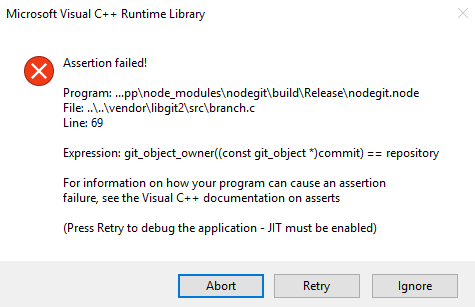
\includegraphics[width=\textwidth]{sections/nodegit/images/branch.png}
	\caption{Chybová hláška}
\end{figure}
\FloatBarrier

\section{Git status}

Na obrazovce uživatelského rozhraní Aplikace pro vytvoření nového commitu se mohou zobrazovat tři různé druhy souborů. Změněné soubory jsou buď připravené pro commit, nebo nejsou a v repozitáři jsou známé či neznámé.

\subsection{Odebrání smazaného souboru}

NodeGit poskytuje pro přidávání do a odebírání z připravených položek (staging area) dvě metody, \mintinline{javascript}{Index.add(path)} a \mintinline{javascript}{Index.remove(path)}. Obě metody přijímají přijímají jako argument cestu, řetězec znaků, které určují polohu souboru v lokálním souborovém systému. V obou případech dochází k chybě při manipulaci se souborem, který se v systému již nenachází. Pomocí těchto metod tedy nejde pracovat s přidávání a odebíráním neexistujících souborů na a ze stage. Alternativu NodeGit nenábízí. Řešením je tedy systémové volání v JavaScriptu, které umožňuje přístup k příkazovému řádku, na které lze spouště příkazy \mintinline{bash}{git}. Pro fungování tohoto postupu je nutná instalace programu git a přidání do systémové cesty pro spustitelné programy na zařízení uživatele.

\FloatBarrier
\begin{figure}[h]
	\begin{minted}[]{javascript}
const exec = require('child-process-promise').exec
exec(`cd ${projectPath} && git add "${filePath}"`))
	\end{minted}
	\caption{Přidání smazaného souboru}
\end{figure}
\FloatBarrier

\subsection{Výpis neznámých}

% @TODO: http://www.nodegit.org/api/repository/ https://github.com/nodegit/nodegit/tree/master/examples
Se smazanými soubory má problémy i metoda na zjištění změněných souborů \mintinline{javascript}{Repository.getStatus()}. Pro smazané, případně přejmenované, soubory vrací neúplná data, se kterými není možné dále pracovat. Stejně jako v předchozím bodě, dokumentace a ukázky NodeGitu nepočítají s odstraněnými soubory. V tomto případě je však mezi uživateli známo náhradní řešení, které pomocí metody \mintinline{javascript}{Diff.indexToWorkdir(...)} vyhledá všechny změněné neignorované soubory či adresáře a vrátí jejich cesty, se kterými lze dále snadno pracovat pomocí systémových volání \mintinline{bash}{git add path} či \mintinline{bash}{git reset HEAD path}.

\section{Konflikty}

Během slučování stavu na vzdáleném serveru a stavu v lokálním repozitáři může dojít ke kolizím v případě, že například oba stavy obsahují v historii nové změny stejného souboru na stejných řádcích. V takovém případě je nutno rozhodnout, které změny zůstanou po sloučení, případně typicky uživatel má možnost ručně udělat změny nové, které berou oba zdroje v potaz. Aplikace automaticky preferuje změny ze vzdáleného repozitáře, což je omezení nedokonalosti metod NodeGitu pro slučování, které může vést ke nezpozorované ztrátě změn či k nevalidnímu kódu projektu. Proto Aplikace na toto nebezpečí upozorňuje po sloučení zprávou ve Snackbaru. NodeGit při výskytu kolize udržuje stav souborů pouze v paměti, což omezuje uživatelovi možnosti, jak nesrovnalosti napravit. Pravděpodobně nejlepším řešením by bylo promítnout soubory do souborového systému, aby je uživatel mohl upravit ve vlastním editoru, jako se to běžné dělá při klasickém používání příkazu \mintinline{bash}{git merge} či \mintinline{bash}{git pull}.

\section{Autentizace}

\subsection{Vzdálené servery}

% @TODO

\subsection{Uložiště přístupových údajů}

% @TODO

\subsection{Správce klíčů pro SSH}

% @TODO

\subsection{cURL}

% @TODO


\chapter{Návrhy na rozšíření}

Zejména kvůli nedostatkům pro tuto práci klíčové knihovny NodeGit nebylo možné v omezeném čase postihnout veškeré neduhy výsledné Aplikace, které byly objeveny během vývoje či při uživatelském testování. Následující přehled by měl navrhnout jejich řešení, případně doplnit Aplikaci o další funkcionalitu, která by aplikaci významně prospěla.


\section{Zlepšení stávajících funcionalit}

\subsection{Nezobrazovat příliš obsáhlé změny}

U ručně psaných textů se jedná sice spíše o okrajový problém, avšak u projektů, kde uživatel přidává do projektů například celé knihovny či generované texty, se může stát, že množství těchto textů bude příliš náročné na vypsání do okna aplikace například v detailu commitu. Taková zátěž může způsobit nežádoucí pomalý běh aplikace či její úplné zamrznutí. Bylo by tedy vhodné takovým situacím předcházet. Například u větších změn zobrazovat jen kratší název a zbytek až na vyžádání uživatele například stiskem nějakého tlačítka „zobrazit více“.

\subsection{Zobrazovat celou historii}

Obrazovka s historií projektu nyní zobrazuje jen commity do maximálního počtu 250. Tento limit zaručuje u projektů s bohatou historií plynulý chod za cenu toho, že uživatel starší commity nevidí. Vzhledem k tomu, že plynulost je potřeba zachovat, bylo by vhodné uživateli nabídnout alespoň stránkování, aby se nevypisovaly všechny commity naráz, nebo implementovat chytřejší vykreslování, které by budilo dojem souvislé historie i přes omezení množství commitů, které mohou být v jeden okamžit načteny do grafického rozhraní, které je tím nejslabším článkem při práci s větším množstvím dat.

\subsection{Chytřejší upozorňování na vytvoření commitu}

Aktuální upozorňovací mechanizmus nebere v potaz hlubší specifika konkrétního projektu. Kromě analýzy počtu přidaných a odebraných řádků a změněných souborů, by bylo vhodné například u projektů psaných zejména v \LaTeX{u} sledovat počet změněných kapitol (chapter) či sekcí (section), aby autor pro dosažení ideálního commitu nezasahoval do příliš mnoha nesouvislých částí projektu. Podobný princip by bylo možné implementovat i pro jiné, například programovací, jazyky. V objektově orientovaných se vybízí přirovnání kapitol k třídám a sekcí k metodám. Představou ideálního commitu budiž takový, který neobsahuje více nesouvislých změn.

\subsection{Průvodce ovládáním}

Uživatelské rozhraní spoléhá na silnou intuici či dřívější zkušenost. Malé množství popisků a terminologie typická pouze pro Git (například „commit“) nikterak neulehčují uživateli orientaci v Aplikaci. Řešením tohoto neduhu by bylo doplnění více popisků ke většině prvků. Popisky by mohli mohly být představeny uživateli ve dvou podobách. První variantou by byly takové, které se zobrazí pouze při prvním setkání uživatele s daným prvkem. Druhé pak stručnější stálé.

\subsection{Přidávání projektu}

Kromě lépe formulovaných a obsáhlejších popisků v modálním okně pro přidávání nového projektu by jistě usnadnily ovládání ukázky typických zástupců online služeb pro správu Gitových repozitářů (například GitHub, Bitbucket, GitLab), jak se v těchto službách zakládají nové projekty a kde je adresa pro remote, která se využívá v Aplikaci právě při přidávání projektu z URL.

\subsection{Stálé menu}

Při větších velikostech hlavního okna, na širších displayích, zůstává větší míra plochy nevyužita. Vzhledem k tomu, že v zasouvacím menu se nachází spoustu pro užívání Aplikace kritických položek, uživatelský zážitek by zlepšilo, kdyby menu zůstalo stále vysunuté po boku ostatního obsahu.

\subsection{Podpora kódování}

% @TODO: obrázek na ukázku
Aplikace pro zobrazování textů používá kódování UTF-8, což může způsobit problémy při zobrazování změn v souborech, které používají kódování jiné. Vzhledem k tomu, že UTF-8 je rozšířením ASCII, aktuálně tento nedostatek nezpůsobuje úplnou nečitelnost, ale některé speciální znaky, v češtině zejména písmena s háčkem nebo čárkou, jsou nahrazena zástupným symbolem s otazníkem. Pro takové případy by bylo vhodné do aplikace doplnit detekci kódování upravených souborů a jejich zobrazování patřičně opravit.

\subsection{Bohatší přehled při začleňování změn}

Obrazovka pro začlenění nových změn obsahuje pouze přehled samotných pozměněných souborů. Užitečnou informací by mohlo pro uživatele být, kdy byly změny vytvořeny, kdo je jejich autorem a z jakých commitů se skládají. Detailnější přehled by vedl k rychleší orientaci při začleňování a lepšímu porozumění konkrétních úprav.

\subsection{Podpis na Windows}

Z bezpečnostních důvodů kontroluje systém Windows podpis autora aplikaci. Přidávání podpisu není zatím v automatické distribuci balíčků začleněno. Uživateli je tak sestémem doporučeno, aby Aplikaci neužíval, což je nežádoucí chování a může vést k tomu, že potenciální uživatel Aplikaci opravdu nespustí. Řešením je tedy registrace vývojáře a začlenění podepisování do vytváření předpřipravených balíčků.


\section{Nové funkcionality}

\subsection{Změna jména a e-mailu}

% @TODO: ukázka git příkazu
Zejména noví uživatelé Gitu nemají často nastaveno jméno a e-mail. Tyto údaje se používají při vytváření commitu a slouží k identifikaci autora. Správně nastavené jméno a heslo například zpřehledňuje historii. Uživatele bez jména a e-mailu by tedy bylo vhodné na tuto skutečnost upozornit a odkázat například do nastavení, kde by jméno a e-mail bylo možné změnit.

\subsection{Zvýraznění syntaxe}

Při volbě vhodných nástrojů pro vývoj Aplikace byl zahrnut i požadavek na možnost zvýrazňování syntaxe, předně \LaTeX{ové}, například na obrazovce s detailem commitu. Pro JavaScript je k dispozici nepřeberné množství knihoven zajišťujícíh tuto funkcionalitu. Při jejich studii byl zvolen CodeMirror\footnote{\url{https://codemirror.net/}} jako nejatraktivnější vzhledem k vestavěné podpoře \LaTeX{u} a možnosti zobrazovat změny v souborech.

\subsection{Náhled obrázků}

Přehled změn zobrazuje pouze textové úpravy. U binárních souborů se ukáže pouze jejich název a typ změny (přidán, změněn, odstraněn). V případě obrázků se tedy vybízí zobrazit navíc i jejich náhled, pro případ, že si uživatel obsah například nepamatuje nebo ho nikdy neviděl, protože pochází od jiného autora.

\subsection{Otevření editoru}

Pro rychlejší práci se soubory by byla užitečná u každé zmínky souboru projektu možnost otevřít ho rovnou ve vlastním editoru, který si uživatel nastavil v operačním systému, aby mohl více času trávit v prostředí, ve kterém samotný osah tvoří. Pro soubory a jejich stavy, které jsou dostupné pouze v historii, by se mohly tvořit dočasné verze, které by nebylo možné upravovat. Pro tuto funkcionalitu bylo zahájeno zkoumání, jehož výsledkem bylo odložení implementace kvůli příliš rozličnému chování různých operačních systému.

\subsection{Označování commitů}

V některých projektech bývá zvykem používat takzvané tagy, značky, kterými je možné označit libovolný commit doplňujícím textem pro snazší orientaci v historii či pro doplnění commitu o další informaci. Například v repozitáři se zdrojovými kódy Aplikace se tagy využívájí pro označení commitů, pro které se mají automaticky vytvořit předpřipravené balíčky pro snadné stažení. Pro podporu tagů je potřeba minimálně v obrazovce historie zobrazovat již existující tagy a přidat možnost jejich vytvoření pro libovolný commit, zároveň doplnit logiku pro jejich synchronizaci.

\subsection{Změna větve}

Další často využívanou funkcí Gitu při práci zejména ve vícech lidech je přepínání větví. Jejich přehled a změna je rozpracován v zobrazení detailu projektu, ale kvůli současné nedokončé implementaci možnosti začlenit větev do větve jiné je tento přehled zatím skryt. Doplnění práce s větvemi by také vyžadovalo změnit přístup zobrazovaní historie, který momentálně s cílem zpřehlednění strukturu větví potlačuje.

\subsection{Kontrola závislostí}

Aplikace se spoléhá na některé další programy, které musí být v systému nainstalovány a správně nastaveny. Pro správné fungování by měla Aplikace kontrolovat, že všechny tyto závislosti jsou dostupné. Jedná se zejména o Git a jeho podpůrné nástroje například pro správu přístupových údajů, Credential Store a Pageant. V případě nedostupnosti či špatné konfigurace by měla Aplikace na tuto skutečnost uživatele upozornit s nápovědou možného řešení.

\subsection{Propojení se vzdálenými servery}

% @TODO: co s issues?
Servery jako GitHub, Bitbucket, GitLab nabízejí vlastní bohaté rozhraní na správu projektů. Některé funkce představují pouze alternativu (detail commitu, základní historie) a jiné doplněk k Aplikaci (issues). Toto propojení není vhodné skrývat, nýbrž podporovat, protože uživateli nabízí více pomocných nástrojů pro snadnější práci na projektu. Kromě odkazování se na tyto servery při přidávání projektů by měla podobná vazba existovat i mezi jednotlivými commity, kdy pomocí hashe commitu je snadné automaticky složit odpovídající URL pro běžně používané servery a nabídnout uživatelovi tedy přechod na přání do internetového prohlížeče.

\subsection{Hlášení chyb uživatelovi}

Například během připojování ke vzdálenému serveru může dojít k mnoha různým chybám, o kterých nyní není uživatel nikterak informován. Často se jedná o chyby, které se týkají zamezení přístupu k projektu, protože má uživatel špatně nastavené heslo, špatný nebo žádný klíč pro SSH, přístup mu nebyl nikdy udělen, není připojen k internetu apod. O chybách je možné uživatele informovat třeba pomocí systémových upozornění či komponentou Snackbar [Obrázek \ref{fig:snackbar}]. Je však nutné se najdříve vypořádat se zpracováním chyb, které jsou knihovnou NodeGit často předávány pouze v textové podobě bez dokumentace; na strojově čitelnější variantě, která je zatím označena jako \uv{EXPERIMENTAL}, se pracuje \cite{nodegit-error-codes}. Další hůře zpracovatelné chyby jsou přímo od vzdálených serverů, které také nejsou možné zobrazit uživateli bez předzpracování, protože nejsou česky, pro nezkušeného uživatele nemají dostatečnou informační hodnotu a formou se liší napříč různými servery, různé texty pro stejné chyby.

\subsection{Hlášení chyb vývojáři}

Za běhu Aplikace může dojít i k chybám, které nemusí oznámením uživateli prospět. Typicky jsou to takové, jež jsou způsobené chybou v kódu, uživateli nejsou zřejmé, neomezují další chod Aplikace. Nyní se takové události zapisují do souboru na uživatelově počítači. Pro možnou analýzu těchto dat je tedy nutné informovat uživatele o jejich extistenci a umožnit jim snadné sdílení s vývojářem třeba e-mailem nebo je odesílat automaticky. Za zvážení stojí i rozhodnutí, jak se vypořádat s chybami, které jsou mimo kontrolu Aplikace. Během vývoje došlo jednou k selhání\footnote{\url{https://github.com/Onset/FitGit/issues/56}} knihovny libgit2\footnote{\url{https://libgit2.github.com/}} napsané v jazyce C, jež po svém pádu nevrátila řízení JavaScriptu, který by chybu mohl zapsat do příslušného souboru. Není vyloučeno, že podobná selhání se mohou opakovat.

\subsection{Ukázkový projekt}

Pro rychlejší pochopení uživatelského rozhraní a možnost vyzkoušet si funkce na projektu bez nutnosti vlastního účtu na některé ze služeb poskytujících správu repozitářů by bylo užitečné po prvním spuštění Aplikace nabídnout uživatelovi ukázkový projekt, kde by si mohl vyzkoušet, jak s projektem pracovat či otestovat, jestli mu Aplikace vyhovuje.


\section{Ostatní zlepšení}

\subsection{Verze pro macOS}

Electron a NodeGit, jenž jsou základním stavebním kamenem Aplikace, jsou otevřeny pro široké spektrum operačních systémů, do kterého patří i macOS. Vzhledem k tomu, že Aplikace není závislá na ničem, co by princip této dostupnosti nesdílelo, přímo se vybízí tuto platformu začlenit do automatického procesu vytváření předpřipravených balíčků. Dokonce v některých fázích vývoje aplikace k této automatizaci docházelo, avšak kvůli některým odlišnostem od ostatních systémů od toho bylo upuštěno kvůli příliš rychlým iteracím při vývoji, kdy tím pádem bylo potřeba udržovat průběžnou integraci pro tři systémy, což v době rapidního vývoje jevilo časově nevýhodné. Nyní je Aplikace v ustálenějším stavu a začlenění macOS by tedy nemělo způsobovat větší komplikace.

\subsection{A další}

Předchozí body jsou pouze výňatkem těch pravděpodobně nejzásádnějších změn a rozšíření, které by Aplikaci pomohly k úspěchu mezi možnými uživateli. Podobných zlepšení je více a některé mohou teprve vyvstat po rozšíření mezi více lídí. Mimo to se i stále vyvýjí prostředí, se kterým Aplikace pracuje. Operační systémy, Git, Electron, NodeGit, GitHub, Bitbucket, GitLab se stále posouvají kupředu, tudíž pro optimální fungování je potřeba s nimi držet krok.

\chapter{Realizace}

\begin{conclusion}
	%sem napište závěr Vaší práce
	Bakalářská práce je momentálně již rozpracovaná. Byl proveden průzkum mezi šesti učiteli, kteří v LaTeXu běžně tvoří obsah v týmu. V rozhovorech se všichni shodli, že aktuální stav není ideální a až na jednoho člověka by všichni ocenili lepší, přehlednější řešení. Mimo to byly také prozkoumány alternativní nástroje, které jsou ve spojení LaTeXu a spolupráce známé, ale nikdo z tázaných s nimi neměl zkušenost. Konkrétně se jednalo o webové služby ShareLaTeX [2] a Overleaf {cit4}. Závěrem je potvrzení, že má smysl nové řešení vyvíjet a zároveň došlo k jeho detailnější specifikaci.
\end{conclusion}

\bibliographystyle{csn690}
\bibliography{mybibliographyfile}

\appendix

\chapter{Seznam použitých zkratek}
% \printglossaries
\begin{description}
	% @TODO: doplnit IRC, URL, SSH, UI
	
	% @TODO: odebrat GUI a XML - jen ukázky
	\item[GUI] Graphical user interface
	\item[XML] Extensible markup language
\end{description}


% % % % % % % % % % % % % % % % % % % % % % % % % % % %
% % Tuto kapitolu z výsledné práce ODSTRAŇTE.
% % % % % % % % % % % % % % % % % % % % % % % % % % % %
%
% \chapter{Návod k~použití této šablony}
%
% Tento dokument slouží jako základ pro napsání závěrečné práce na Fakultě informačních technologií ČVUT v~Praze.
%
% \section{Výběr základu}
%
% Vyberte si šablonu podle druhu práce (bakalářská, diplomová), jazyka (čeština, angličtina) a kódování (ASCII, \mbox{UTF-8}, \mbox{ISO-8859-2} neboli latin2 a nebo \mbox{Windows-1250}).
%
% V~české variantě naleznete šablony v~souborech pojmenovaných ve formátu práce\_kódování.tex. Typ může být:
% \begin{description}
% 	\item[BP] bakalářská práce,
% 	\item[DP] diplomová (magisterská) práce.
% \end{description}
% Kódování, ve kterém chcete psát, může být:
% \begin{description}
% 	\item[UTF-8] kódování Unicode,
% 	\item[ISO-8859-2] latin2,
% 	\item[Windows-1250] znaková sada 1250 Windows.
% \end{description}
% V~případě nejistoty ohledně kódování doporučujeme následující postup:
% \begin{enumerate}
% 	\item Otevřete šablony pro kódování UTF-8 v~editoru prostého textu, který chcete pro psaní práce použít -- pokud můžete texty s~diakritikou normálně přečíst, použijte tuto šablonu.
% 	\item V~opačném případě postupujte dále podle toho, jaký operační systém používáte:
% 	\begin{itemize}
% 		\item v~případě Windows použijte šablonu pro kódování \mbox{Windows-1250},
% 		\item jinak zkuste použít šablonu pro kódování \mbox{ISO-8859-2}.
% 	\end{itemize}
% \end{enumerate}
%
%
% V~anglické variantě jsou šablony pojmenované podle typu práce, možnosti jsou:
% \begin{description}
% 	\item[bachelors] bakalářská práce,
% 	\item[masters] diplomová (magisterská) práce.
% \end{description}
%
% \section{Použití šablony}
%
% Šablona je určena pro zpracování systémem \LaTeXe{}. Text je možné psát v~textovém editoru jako prostý text, lze však také využít specializovaný editor pro \LaTeX{}, např. Kile.
%
% Pro získání tisknutelného výstupu z~takto vytvořeného souboru použijte příkaz \verb|pdflatex|, kterému předáte cestu k~souboru jako parametr. Vhodný editor pro \LaTeX{} toto udělá za Vás. \verb|pdfcslatex| ani \verb|cslatex| \emph{nebudou} s~těmito šablonami fungovat.
%
% Více informací o~použití systému \LaTeX{} najdete např. v~\cite{wikilatex}.
%
% \subsection{Typografie}
%
% Při psaní dodržujte typografické konvence zvoleného jazyka. České \uv{uvozovky} zapisujte použitím příkazu \verb|\uv|, kterému v~parametru předáte text, jenž má být v~uvozovkách. Anglické otevírací uvozovky se v~\LaTeX{}u zadávají jako dva zpětné apostrofy, uzavírací uvozovky jako dva apostrofy. Často chybně uváděný symbol "{} (palce) nemá s~uvozovkami nic společného.
%
% Dále je třeba zabránit zalomení řádky mezi některými slovy, v~češtině např. za jednopísmennými předložkami a spojkami (vyjma \uv{a}). To docílíte vložením pružné nezalomitelné mezery -- znakem \texttt{\textasciitilde}. V~tomto případě to není třeba dělat ručně, lze použít program \verb|vlna|.
%
% Více o~typografii viz \cite{kobltypo}.
%
% \subsection{Obrázky}
%
% Pro umožnění vkládání obrázků je vhodné použít balíček \verb|graphicx|, samotné vložení se provede příkazem \verb|\includegraphics|. Takto je možné vkládat obrázky ve formátu PDF, PNG a JPEG jestliže používáte pdf\LaTeX{} nebo ve formátu EPS jestliže používáte \LaTeX{}. Doporučujeme preferovat vektorové obrázky před rastrovými (vyjma fotografií).
%
% \subsubsection{Získání vhodného formátu}
%
% Pro získání vektorových formátů PDF nebo EPS z~jiných lze použít některý z~vektorových grafických editorů. Pro převod rastrového obrázku na vektorový lze použít rasterizaci, kterou mnohé editory zvládají (např. Inkscape). Pro konverze lze použít též nástroje pro dávkové zpracování běžně dodávané s~\LaTeX{}em, např. \verb|epstopdf|.
%
% \subsubsection{Plovoucí prostředí}
%
% Příkazem \verb|\includegraphics| lze obrázky vkládat přímo, doporučujeme však použít plovoucí prostředí, konkrétně \verb|figure|. Například obrázek \ref{fig:float} byl vložen tímto způsobem. Vůbec přitom nevadí, když je obrázek umístěn jinde, než bylo původně zamýšleno -- je tomu tak hlavně kvůli dodržení typografických konvencí. Namísto vynucování konkrétní pozice obrázku doporučujeme používat odkazování z~textu (dvojice příkazů \verb|\label| a \verb|\ref|).
%
% \begin{figure}\centering
% 	
\includegraphics[width=0.5\textwidth, angle=30]{cvut-logo-bw}
% 	\caption[Příklad obrázku]{Ukázkový obrázek v~plovoucím prostředí}\label{fig:float}
% \end{figure}
%
% \subsubsection{Verze obrázků}
%
% % Gnuplot BW i barevně
% Může se hodit mít více verzí stejného obrázku, např. pro barevný či černobílý tisk a nebo pro prezentaci. S~pomocí některých nástrojů na generování grafiky je to snadné.
%
% Máte-li například graf vytvořený v programu Gnuplot, můžete jeho černobílou variantu (viz obr. \ref{fig:gnuplot-bw}) vytvořit parametrem \verb|monochrome dashed| příkazu \verb|set term|. Barevnou variantu (viz obr. \ref{fig:gnuplot-col}) vhodnou na prezentace lze vytvořit parametrem \verb|colour solid|.
%
% \begin{figure}\centering
% 	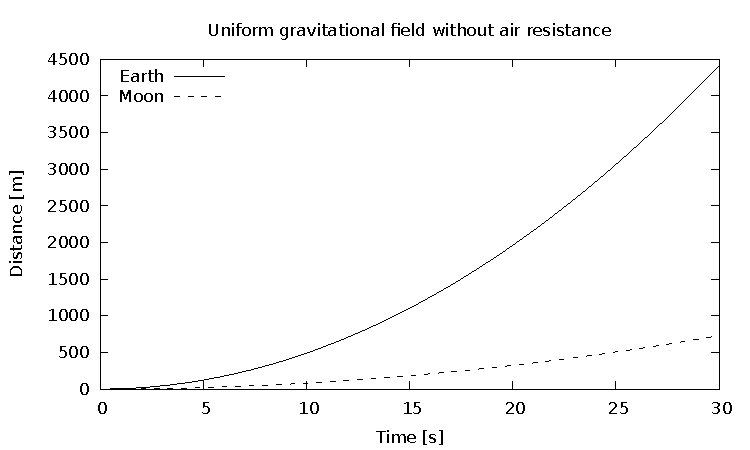
\includegraphics{gnuplot-bw}
% 	\caption{Černobílá varianta obrázku generovaného programem Gnuplot}\label{fig:gnuplot-bw}
% \end{figure}
%
% \begin{figure}\centering
% 	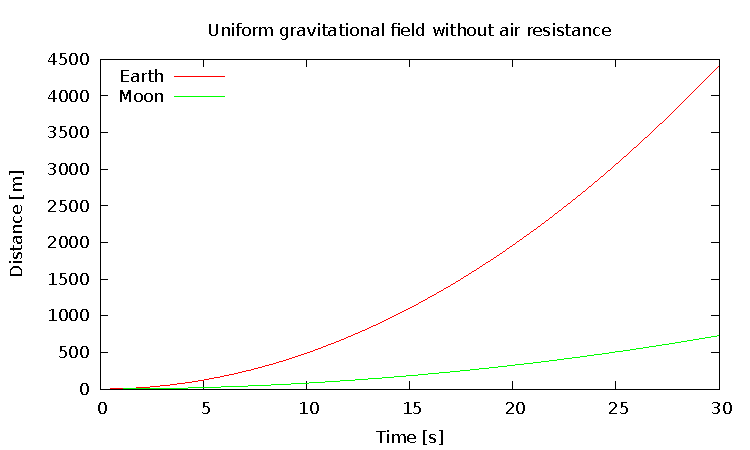
\includegraphics{gnuplot-col}
% 	\caption{Barevná varianta obrázku generovaného programem Gnuplot}\label{fig:gnuplot-col}
% \end{figure}
%
%
% \subsection{Tabulky}
%
% Tabulky lze zadávat různě, např. v~prostředí \verb|tabular|, avšak pro jejich vkládání platí to samé, co pro obrázky -- použijte plovoucí prostředí, v~tomto případě \verb|table|. Například tabulka \ref{tab:matematika} byla vložena tímto způsobem.
%
% \begin{table}\centering
% 	\caption[Příklad tabulky]{Zadávání matematiky}\label{tab:matematika}
% 	\begin{tabular}{|l|l|c|c|}\hline
% 		Typ		& Prostředí		& \LaTeX{}ovská zkratka	& \TeX{}ovská zkratka	\tabularnewline \hline \hline
% 		Text		& \verb|math|		& \verb|\(...\)|	& \verb|$...$|		\tabularnewline \hline
% 		Displayed	& \verb|displaymath|	& \verb|\[...\]|	& \verb|$$...$$|	\tabularnewline \hline
% 	\end{tabular}
% \end{table}
%
% % % % % % % % % % % % % % % % % % % % % % % % % % % %

\chapter{Obsah přiloženého CD}

%upravte podle skutecnosti

\begin{figure}
	\dirtree{%
		.1 readme.txt\DTcomment{stručný popis obsahu CD}.
		.1 exe\DTcomment{adresář se spustitelnou formou implementace}.
		.1 src.
		.2 impl\DTcomment{zdrojové kódy implementace}.
		.2 thesis\DTcomment{zdrojová forma práce ve formátu \LaTeX{}}.
		.1 text\DTcomment{text práce}.
		.2 thesis.pdf\DTcomment{text práce ve formátu PDF}.
		.2 thesis.ps\DTcomment{text práce ve formátu PS}.
	}
\end{figure}

\end{document}
